%% LyX 2.3.1-1 created this file.  For more info, see http://www.lyx.org/.
%% Do not edit unless you really know what you are doing.
\documentclass[english,hebrew]{article}
\usepackage[T1]{fontenc}
\usepackage[utf8]{inputenc}
\usepackage{babel}
\usepackage{graphicx}
\usepackage[unicode=true]
 {hyperref}
\begin{document}
\title{אז מה הקטע עם אחוזים?}
\maketitle
\begin{description}
\item [{קטגוריות:}] כללי
\item [{תגים:}] אחוזים
\item [{מזהה:}] \L{what\_are\_percents}
\end{description}
המוטיבציה לפוסט הזה היא חברה כלשהי שהציעה 'מבצע ללא מע\textquotedblleft מ'
שנותן הנחה של \L{$14.5\%$} על מוצריה. אלא מה, אחוז המע\textquotedblleft מ
בישראל כרגע הוא \L{$17\%$} ואיך שלא תסתכלו על זה, \L{$14.5$} ו-\L{$17$}
הם ככל הנראה לא אותם מספרים. \textbf{יותר גרוע}, \L{$14.5$} הוא מספר
\textbf{קטן יותר} מאשר \L{$17$} כך שריח חמור של הונאה עולה באפינו!
החברה הפיקחית חזתה את ההתנגדות הזו מראש וצירפה דברי הבהרה שמסבירים
ומדגימים שהנחה של \L{$17\%$} הייתה \textbf{גדולה מדי} במקרה הזה.
האם מה שהם כותבים היה ברור? אשאיר לכן את השיפוט:

\textbf{\L{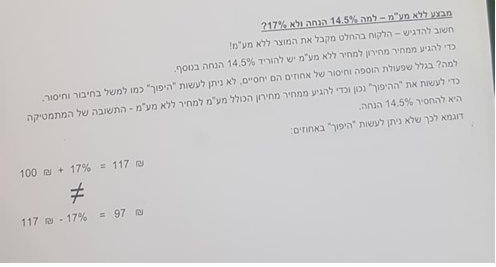
\includegraphics{C:/Users/GADIALEKSANDROWICZ/Dropbox/Websites/blog/assets/img/2020/01/percent_discount}}}

אני רוצה לנצל את ההזדמנות כדי להסביר מה זה אחוזים, למה החברה צודקת
בחשבון שאלה ומאיפה המספר הקסום העגול והיפה \L{$14.5$} צץ אל הקיום
שלנו מתוך \L{$17$} )ספוילר: זה לא \L{$14.5$} אלא \L{$14.529914529914\dots$}(.

אז מה זה אחוזים? הרעיון באחוזים הוא לקחת \textbf{משהו} ולחלק אותו
ל-{\beginL 100\endL} חלקים שווים בגודלם, ואז \textquotedblright אחוז\textquotedblleft{}
בודד הוא אחד מבין החלקים הללו. למה דווקא המספר {\beginL 100\endL}?
זה שרירותי לגמרי. אפשר היה בתיאוריה גם לחלק ל-{\beginL 10\endL} חלקים,
או {\beginL 1,000\endL}, או {\beginL 137\endL} או {\beginL 42\endL}.
אבל {\beginL 100\endL} הוא מספר טוב כי הוא לא גדול ולא קטן מדי לצרכים
שבהם בדרך כלל משתמשים באחוזים, והוא עגול )\L{\href{https://gadial.net/2017/06/11/number_bases/}{בבסיס}}
{\beginL 10\endL}, אבל זה הבסיס שבו אנחנו משתמשים בחיי היומיום שלנו(.

איפה משתמשים בזה? בשלל מקומות בחיי היום-יום. זה אחד מהמושגים המתמטיים
הנפוצים ביותר מחוץ למתמטיקה עצמה. הנה דוגמא קלאסית - מד התקדמות:

\textbf{\L{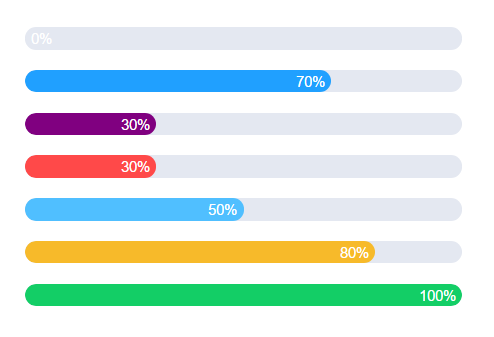
\includegraphics{C:/Users/GADIALEKSANDROWICZ/Dropbox/Websites/blog/assets/img/2020/01/progress_bar}}}

במד התקדמות משתמשים כשיש יעד כלשהו שרוצים להגיע אליו )החל בטעינה של
תוכנית מחשב וכלה בלמידה של קורס שפה חדשה( ורוצים לתת ייצוג ויזואלי
להתקדמות שלנו בו, בדמות פס שחלק ממנו מלא )האיזורים הצבעוניים בתמונה(
וחלק ממנו עדיין ריק. לרוב הייצוג הויזואלי הזה ילווה גם באחוזים שנותנים
את הכמות המדוייקת מהפס שכבר מלאה. כך \L{$50\%$} מציינים שבדיוק חצי
ממד ההתקדמות מלא )כי \L{$50$} הוא חצי מ-\L{$100$}, שהרי \L{$\frac{50}{100}=\frac{1}{2}$}(,
\L{$100\%$} מציינים שכל מד ההתקדמות מלא, וכן הלאה.

טוב ויפה, אבל דוגמת מד ההתקדמות שלי היא גם כזו שלא \textbf{חייבים}
בה אחוזים - אם נשמיט את המספרים עדיין נקבל ייצוג ויזואלי נחמד שעומד
בפני עצמו. אחוזים הם מועילים יותר כשאנחנו רוצים לקבל מידע מדויק יותר.
למשל, על מיסים או הנחות, כמו בדוגמא שממנה התחלנו. נתחיל עם המס. מה
זה אומר, מס ערך מוסף של \L{$17\%$}? בפועל זה אומר שאם המחיר של משהו
היה \L{$X$}, אז למחיר הזה צריך להוסיף עוד שבע-עשרה אחוזים ממנו כדי
להגיע למחיר שאותו נשלם בפועל. כלומר, המחיר יהיה \L{$X+\frac{17}{100}X=\left(1+\frac{17}{100}\right)X=\frac{117}{100}X$}.

הנה עוד דרך לומר את זה: אחרי שמוסיפים למשהו \L{$17\%$} של מס, המחיר
שלו יעלה ויגיע לרמה של \L{$117\%$} ממחירו המקורי. כלומר, ייקור של
משהו בעקבות מס ניתן לתיאור על ידי כפל של המשהו במספר שמתאר את ההתייקרות.
באופן דומה גם \textbf{הנחה} במשהו ניתנת לתיאור באמצעות כפל. נניח,
הנחה של \L{$25\%$} ניתנת לתיאור בתור \L{$X-\frac{25}{100}X=\frac{75}{100}X$}.

אצלי הדבר הזה יוצר מייד בלבול - הרי כפל בדברים מקיים את \textbf{חוק
החילוף}, כלומר לא משנה במה כופלים קודם. אם אני כופל את \L{$X$} ב-\L{$2$}
ואז ב-\L{$5$} זה אותו דבר כמו לכפול אותו קודם ב-\L{$5$} ואז ב-\L{$2$}.
אז אם הנחה/מס שניהם מתבטאים על ידי כפל, למה הם לא מתחלפים ביניהם?
התשובה היא שהם כן, פשוט לא באופן שאני מצפה לו אינטואיטיבית. בואו נראה
דוגמת צעצוע עם מספרים נחמדים כדי לראות את זה.

נניח שפריט מסויים עולה {\beginL 100\endL} ש\textquotedblleft ח. בנוסף
לכך מעורבים בסיפור מע\textquotedblleft מ של \L{$20\%$} )כדי שיהיה
עגול( והנחה של \L{$50\%$}. אם שואלים אתכן מה אתן מעדיפות קודם - לקבל
את ההנחה או לחטוף את המס - התשובה היא שזה באמת לא משנה מה יבוא קודם.
אם קודם יינתן המע\textquotedblleft מ, אז מחיר הפריט יקפוץ ל-{\beginL 120\endL}
ש\textquotedblleft ח, ואחרי ההנחה הוא יירד ל-{\beginL 60\endL} ש\textquotedblleft ח;
ואם קודם תינתן ההנחה אז מחיר הפריט יירד ל-{\beginL 50\endL} ש\textquotedblleft ח
ואחרי המע\textquotedblleft מ הוא יקפוץ ל-{\beginL 60\endL} ש\textquotedblleft ח.
כלומר, חוק החילוף אומר שלא משנה באיזה סדר אני מפעיל את השינוי-באחוזים,
התוצאה הסופית תהיה זהה. אבל הוא לא אומר ולא מנסה לומר שהעלאת מחיר
והורדת מחיר באותו אחוז אמורים להוביל לאפקטים שמבטלים זה את זה. זה
בדיוק מה שנאמר בהסבר שבדף שהראיתי בהתחלה - אין כאן ביטול הדדי בגלל
שבניגוד לחיבור וחיסור \textquotedblright רגילים\textquotedblleft{}
שבהם תמיד מוסיפים את אותו המספר, כאן המספר שמוסיפים/מחסירים הוא \textbf{יחסי}
- הוא תלוי בתוצאת הביניים.

המציאות המתמטית היא שהטבע מוטה מלכתחילה \textbf{בעד} הורדת מחיר. כלומר,
אם מעלים ומורידים את המחיר באותו אחוז, התוצאה הסופית תהיה תמיד נמוכה
יותר ממה שהתחלנו ממנו, אלא אם... עוד רגע נראה אלא אם מה. לפני כן,
הנה דוגמא פשוטה: אם נלך לפריט שמחירו {\beginL 100\endL} ש\textquotedblleft ח
מקודם, וגם נעלה וגם נוריד \L{$50\%$} ממחירו, נקבל {\beginL 75\endL}
ש\textquotedblleft ח )כי או שנעלה מ-{\beginL 100\endL} אל {\beginL 150\endL}
ואז נרד ל-{\beginL 75\endL}, או שנרד מ-{\beginL 100\endL} ל-{\beginL 50\endL}
ואז נעלה ל-{\beginL 75\endL}(. האם יש לי דרך לחשב מתמטית כמה מחיר
הפריט ישתנה מבלי שאצטרף להפעיל את שתי הפעולות בזו אחר זו? כמובן שכן,
בואו נעשה קצת חשבון.

אני אסמן ב-\L{$a$} את האחוז של ההתייקרות/הנחה. זה אומר שאם מחיר הפריט
המקורי היה \L{$X$}, אז כדי לקבל את ההתייקרות שלו נכפול ב-\L{$\frac{100+a}{100}$}
וכדי לקבל את ההנחה שלו נכפול ב-\L{$\frac{100-a}{100}$} וכדי לקבל
את שניהם נכפול בשניהם. עכשיו, יש נוסחה כללית במתמטיקה שאומרת ש-\L{$\left(x+y\right)\left(x-y\right)=x^{2}-y^{2}$}
ואפשר להשתמש בה על \L{$\left(100+a\right)\left(100-a\right)$} ולקבל
שהמחיר החדש של הפריט יהיה \L{$\frac{100^{2}-a^{2}}{100^{2}}X$}. כדי
לפשט את זה טיפה אפשר לחלק את המונה והמכנה ב-{\beginL 100\endL} בריבוע
ולקבל שהמחיר החדש יהיה פשוט \L{$\left(1-\left(\frac{a}{100}\right)^{2}\right)X$}.

שימו לב לכך ש-\L{$\frac{a}{100}$} זה בסך הכל השינוי במחיר כשהוא מיוצג
בתור שבר - במקום נאמר לומר \L{$a=50$} כדי לציין \textquotedblright חמישים
אחוזים\textquotedblleft , \L{$\frac{a}{100}$} אומר \textquotedblright חצי\textquotedblleft .
זו הדרך של היקום המתמטי לרמוז לנו שאחוזים זה משחק נחמד שאנחנו בני
האדם משחקים בינינו לבין עצמנו כי אנחנו אוהבים את המספר {\beginL 100\endL},
אבל הוא לא צריך את זה - {\beginL 100\endL} לא באמת משחק תפקיד במשוואה,
אלא רק השבר שמייצג את ההנחה/התייקרות.

עכשיו, הנוסחה שקיבלנו היא מהצורה \L{$1-\left(\frac{a}{100}\right)^{2}$}.
כלומר, אחד פחות ריבוע של מספר שהוא בין {\beginL 0\endL} ל-{\beginL 1\endL}.
לכן התוצאה תצא בעצמה מספר בין {\beginL 0\endL} ל-{\beginL 1\endL},
ולכן המחיר הסופי תמיד יכול רק לרדת. אם תשאלו אותי איפה הסימטריה הקוסמית
נשברת כך שה\textquotedblleft הנחה\textquotedblleft{} מנצחת את ה\textquotedblleft התייקרות\textquotedblleft ,
זה כבר בנוסחה \L{$\left(x+y\right)\left(x-y\right)=x^{2}-y^{2}$}
שבה בתוצאה הסופית יש מינוס. נקודה אחת שכן כדאי להתייחס אליה הוא שהביטוי
\L{$1-t^{2}$} \textbf{כן} יכול לצאת גדול יותר מ-{\beginL 1\endL}:
בתנאי ש-\L{$t$} יהיה \textbf{מספר מדומה}, למשל \L{$t=2i$} )ואז \L{$1-t^{2}=5$}(.
מה דעתכן, כדאי לתת מע\textquotedblleft מ שמחושב בעזרת מספר מדומה?

טוב, מספיק עם החימום, בואו ניגש לאקשן - אם יש מע\textquotedblleft מ
בשיעור \L{$a$}, כמה גדולה צריכה להיות ההנחה בשיעור \L{$b$} שמקזזת
אותו בדיוק? זה חישוב לא מסובך אבל גם לא לגמרי טריוויאלי.

אנחנו כבר יודעים שמע\textquotedblleft מ בשיעור \L{$a$} פירושו להכפיל
ב-\L{$\frac{100+a}{100}$} )או בעצם, להכפיל ב-\L{$1+\frac{a}{100}$}
- כמו שאמרתי, היקום המתמטי לא מתלהב מה-{\beginL 100\endL} הזה( והנחה
בשיעור \L{$b$} פירושה להכפיל ב-\L{$\frac{100-b}{100}$}. אם שני אלו
מבטלים זה את זו, האפקט צריך להיות \L{$\left(\frac{100+a}{100}\right)\left(\frac{100-b}{100}\right)X=X$}.
אפשר פשוט לחלק ב-\L{$X$} ולקבל 

\L{$\left(\frac{100+a}{100}\right)\left(\frac{100-b}{100}\right)=1$}

עכשיו, אנחנו רוצים לחלץ את \L{$b$} מכל זה. אז קודם כל נכפיל את שני
אגפי המשואוה ב-\L{$\frac{100}{100+a}$} ונקבל

\L{$\frac{100-b}{100}=\frac{100}{100+a}$}

בואו נכפיל ב-{\beginL 100\endL} כדי להיפטר מהמכנה באגף שמאל:

\L{$100-b=\frac{100^{2}}{100+a}$}

נעביר את \L{$b$} אגף ואת מה שבצד ימין אגף:

\L{$100-\frac{100^{2}}{100+a}=b$}

עכשיו נעלה את ה-{\beginL 100\endL} על קו השבר על ידי זה שנכפול אותו
ב-\L{$100+a$}:

\L{$b=\frac{100\left(100+a\right)-100^{2}}{100+a}$}

נפתח סוגריים ונקבל שה-\L{$100^{2}$} מצטמצם ונשארנו עם:

\L{$b=\frac{100a}{100+a}$}

אפשר לעצור פה, אבל שוב - היקום המתמטי לא אוהב את {\beginL 100\endL}.
בואו נחלק ב-{\beginL 100\endL} את המונה והמכנה:

\L{$b=\frac{a}{1+\frac{a}{100}}$}

זה נותן לנו את התשובה באחוזים. אם אנחנו רוצים אותה בשברים יחסיים )כלומר,
\L{$\frac{1}{2}$} במקום {\beginL \L{$50\%$}\endL}ו וכאלה( אפילו
נחלק \textbf{שוב} ב-{\beginL 100\endL}:

\L{$\frac{b}{100}=\frac{a}{100}\cdot\frac{1}{1+\frac{a}{100}}$}

אפשר עכשיו לחזור למקרה של \L{$17\%$} מע\textquotedblleft מ שבו פתחנו.
אם נציב אותו בנוסחה של \L{$b$} שקיבלנו, נקבל:

\L{$b=\frac{17}{1+\frac{17}{100}}=\frac{17}{\frac{117}{100}}=\frac{1700}{117}$}

הביטוי \L{$\frac{1700}{117}$} הוא פשוט... פשוט לא נחמד. אין דרך לפשט
אותו עוד, כי \L{$1700=2^{2}\cdot5^{2}\cdot17$} ו-\L{$117=3^{2}\cdot13$}.
כלומר, אין פה גורמים נוספים שאפשר לצמצם. זה די מבטיח שהייצוג העשרוני
של המספר הזה לא יהיה נחמד. בדיקה במחשבון )או סתם ביצוע תרגיל חילוק
ארוך( תראה שהוא יוצא \L{$14.5299145299\ldots$}, שזה דווקא... די נחמד,
בהתחשב בנסיבות! זה ביטוי מחזורי עם מחזוריות מאוד פשוטה וברורה. אבל
כמובן, אף אחד לא יכתוב ביטוי כל כך ארוך בפועל, אז מסתפקים בלתת הנחה
של \L{$14.5\%$} שהיא... טיפה קטנה יותר ממה שצריך להיות כדי לקזז את
המע\textquotedblleft מ! רמאות! אלא שבפועל, כמובן, ההבדל יבוא לידי
ביטוי בחלקי אגורות שכנראה יעוגלו למטה )אני מקווה( כך שההנחה יוצרת
את אפקט ביטול המע\textquotedblleft מ הדרוש והכל תקין: הציבור קיבל
את ההנחה שמגיעה לו ואני קיבלתי תירוץ לכתוב על אחוזים.
\end{document}
